%UNIT 13: SECOND ORDER LINEAR DEs
%%%%%%%%%%%%%%%%%%%%%%%%%%%
%%%% Put the following at the top of each .tex file  %
\pagestyle{fancy}
\renewcommand{\theUnit}{4.5}
\ifthenelse{\isundefined{\UnitPageNumbers}}{}{\setcounter{page}{1}}
\rhead{Section \theUnit: General Solutions to Nonhomogeneous Second Order Linear DEs}
\lhead{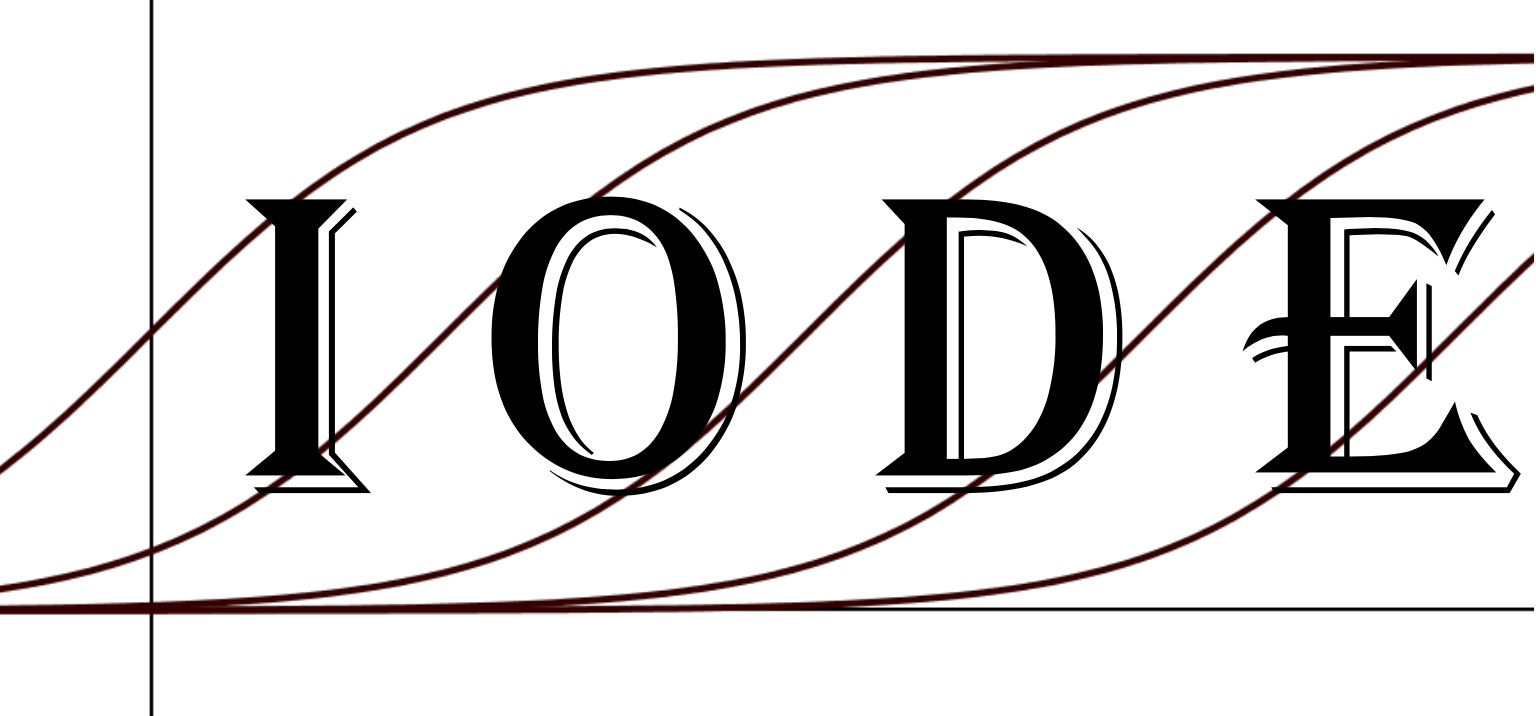
\includegraphics[width=1.25cm]{IODE-logo.png}}
\rfoot{\mypage}
\lfoot{}
\cfoot{}
\fancypagestyle{firstfooter}{\footskip = 50pt}
\renewcommand{\footrulewidth}{.4pt}
%%%%%%%%%%%%%%%%%%%%%%%%%%%
\vspace*{-20pt} \thispagestyle{firstfooter}
\pagebegin{Second Order Linear Differential Equations}

We have developed methods for finding the general homogeneous solution, $y_h(t)$, to a second order differential equation of the form
\[ ay'' + b y' + cy =0 , \ \ \ \ \mbox{for constants $a$, $b$, and $c$}:\]

\bb
\ii Write the differential equation in standard form, $ay'' + b y' + cy =0 $
\ii Set up the corresponding characteristic equation: $ar^2+br+x=0$ and find the roots.
\bi
\ii If two distinct real roots $r_1$ and $r_2$, the general solution is $y_h(t) = C_1e^{r_1t} + C_2e^{r_2t}$.
\ii If one repeated real root $r_1$, the general solution is $y_h(t) = C_1e^{r_1t} + C_2te^{r_1t}$.
\ii If complex solutions $r=\alpha \pm i \beta$, the general solution is $y_h(t) = C_1e^{\alpha t} \cos{(\beta t)} + C_2e^{\alpha t} \sin{(\beta t)}$.
\ei
\ee

We have also discussed how to find the particular solution, $y_p(t)$ to a nonhomogeneous second order differential equation of the form

\[ ay'' + b y' + cy =f(t).\] 

\bb
\ii Based on the form of $f(t)$, we guess $y_p(t)$ will have a similar form.

\begin{center}
\begin{tabular}{|c|c|}
\hline
 & \\
$f(t)$ & $y_p(t)$ \\
 & \\
\hline 
\hline
 & \\
$Ct^n$  (for $n$ a nonnegative integer) &  $A_nt^n + A_{n-1}t^{n-1}+\ldots + A_0 $  \\
 & \\
\hline
 & \\
 $Ce^{rt}$ &  $Ae^{rt}$ \\

%$\dsty Ct^m e^{rt}$ &  $\dsty \left( A_mt^m + A_{m-1}t^{m-1}+\ldots + A_0 \right)e^{rt}$ \\
 & \\
\hline
 & \\
$Ce^{\alpha t} \cos{(\beta t)}$ &  $A e^{\alpha t}\cos{(\beta t)} + B e^{\alpha t}\sin{(\beta t)}$\\
%$\dsty Ct^m e^{\alpha t}\cos{(\beta t)}$ &  $\dsty \bigg( \left( A_mt^m + A_{m-1}t^{m-1}+\ldots + A_0 \right)e^{\alpha t} \cos{(\beta t)}$\\
% & $+ \left( B_mt^m + B_{m-1}t^{m-1}+\ldots + B_0 \right)e^{\alpha t} \sin{(\beta t)} \bigg)$  \\
& \\
\hline
 & \\
 $Ce^{\alpha t} \sin{(\beta t)}$ &  $Ae^{\alpha t} \cos{(\beta t)} + B e^{\alpha t}\sin{(\beta t)}$\\
%$\dsty Ct^m e^{\alpha t}\sin{(\beta t)}$ &  Same as previous case\\
 & \\
\hline
\end{tabular}
\end{center}
\bi
\ii You have \textbf{resonance} when your initial guess for the particular solution is a homogeneous solution.
\ii When there is resonance, multiply the initial guess by $t$ (or $t^2$ if $y_h$ is a solution with a repeated real root).
\ei
\ii Plug your guess into the differential equation, and solve for the undetermined coefficients.
\ee

\clearpage
\pagebegin{Finding the General Solution to the Nonhomogeneous Case}
\bb
\ii Consider the nonhomogeneous differential equation
\[ a y''+by'+cy=f(t).\]
Let $y_h(t)$ denote the general solution to corresponding homogeneous equation $a y''+by'+cy=0$ and let $y_p(t)$ denote the particular solution for the nonhomogeneous equation. \textbf{Show that the function $y(t)=y_h(t)+y_p(t)$ is a solution to the nonhomogeneous differential equation.} \vfill

\ii Consider the differential equation
\[ \frac{d^2x}{dt^2}-\frac{dx}{dt}-12x=e^{4t}.\]
\bb
\ii Find the general homogeneous solution. \vspace{2in}
\ii Find the particular solution to the nonhomogeneous differential equation. \vfill
\ii Give the general solution to nonhomogeneous differential equation.  \vspace{1in}
\ee
\ee

\clearpage
\pagebegin{Breaking Up Sums in the Nonhomogeneous Function}

To find the general solution to the nonhomogeneous differential equation you simply add the particular solution to the general solution to the corresponding homogeneous equation. This 3-step strategy:
\bi
\ii Find the general solution to the corresponding homogeneous equation
\ii Find the particular solution to the nonhomogeneous equation
\ii Add the previous results
\ei
is called the \textbf{Method of Undetermined Coefficients}.


\begin{enumerate}[resume]
\ii Let $y_1(t)$ denote the particular solution to $ay''+by'+cy=f_1(t)$ and $y_2(t)$ denote the particular solution to $ay''+by'+cy=f_2(t)$. Show that $y_p(t) = y_1(t) + y_2(t)$ is the particular solution to $ay''+by'+cy=f_1(t)+f_2(t)$. \vfill


\ii Consider the differential equation
\[ \frac{d^2x}{dt^2}+10\frac{dx}{dt}+9x=85\sin(2t)+18.\]
Recall that we have already worked on parts of this problem. We have found that $x_h (t) = C_1e^{-9t}+C_2e^{-t}$ and the particular solution of $f_1(t) = 85\sin(2t)$ is $x_{1}(t) = -4\cos{(2t)}+\sin{(2t)}$. Using these results, finish solving the differential equation and give the general solution. \vfill

\end{enumerate}

\clearpage

\pagebegin{Products of Different Forms}

We can use the method of undetermined coefficients when the forcing function $f(t)$ is:
\bi
\ii A power function, $f(t) = Ct^n$ (for $n$ a nonnegative integer).
\ii A function of the form $f(t) = Ce^{\alpha t}\cos{(\beta t)}$ or $f(t) = Ce^{\alpha t}\sin{(\beta t)}$.
\ei

\bi
\ii For a product of a power function $t^n$ and an exponential such as $f(t) = Ct^ne^{rt}$, we guess
\[ y_p(t) = (A_n t^n + A_{n_1} t^{n-1} + \ldots A_1 t + A_0)e^{rt}\]
\bi
\ii Multiply by $t$ if $r$ is a real root  (not repeated) of the the characteristic equation.
\ii Multiply by $t^2$ if $r$ is a repeated real root of the the characteristic equation.
\ei \bs
\ei

\bb[resume]
\ii Give a guess for the particular solution to
\[ y'' - 5y' -6y = 4t^2e^{6t}.\] \vfill
\ee


%\ii For a product of an exponential and either a sine or cosine such as $f(t) = Ce^{\alpha t}\cos{(\beta t)}$ or \newline $f(t) = Ce^{\alpha t}\sin{(\beta t)}$, we guess
%\[ y_p(t) =Ae^{\alpha t}\cos{(\beta t)} + Be^{\alpha t}\sin{(\beta t)} \]
%\bi
%\ii Multiply by $t$ if $\alpha \pm i \beta$  are the complex roots of the the characteristic equation.
%\ei \vfill
%\ii For a product of a power function $t^n$ and either a sine or cosine such as $f(t) = Ct^n\cos{(\beta t)}$ or \newline $f(t) = Ct^n\sin{(\beta t)}$, we guess
%\[ y_p(t) =(A_n t^n + A_{n_1} t^{n-1} + \ldots A_1 t + A_0)\cos{(\beta t)} + (B_n t^n + B_{n_1} t^{n-1} + \ldots B_1 t + B_0)\sin{(\beta t)} \]
%\bi
%\ii Multiply by $t$ if $0 \pm i\beta$  are the complex roots of the the characteristic equation.
%\ei \vfill
\bi
\ii For a product of a power function, an exponential, and either a sine or cosine such as \newline $f(t) = Ct^ne^{\alpha t}\cos{(\beta t)}$ or $f(t) = Ct^ne^{\alpha t}\sin{(\beta t)}$, we guess
\[ y_p(t) =(A_n t^n + A_{n_1} t^{n-1} + \ldots A_1 t + A_0)e^{\alpha t}\cos{(\beta t)} + (B_n t^n + B_{n_1} t^{n-1} + \ldots B_1 t + B_0)e^{\alpha t}\sin{(\beta t)} \]
\bi
\ii Multiply by $t$ if $\alpha \pm i \beta$  are the complex roots of the the characteristic equation.
\ei \bs
\ei

\bb[resume]
\ii Give a guess for the particular solution to
\[ y'' - 5y' -6y = 4t^2e^{6t}\sin{t}.\] \vfill
\ee


\clearpage

\begin{enumerate}[resume]

\ii Consider the differential equation $x''-8x'+12x=f(t)$. For each $f(t)$, what would be your guess for the particular solution? Do not solve for the undetermined coefficients. If the method of undetermined coefficients cannot be applied, explain why not.

\bb
\ii $f(t) = 10\sin{(2t)}$ \vfill

\ii $f(t) = 10e^{6t}\sin{(2t)}$ \vfill

\ii $f(t) = 10\tan{(2t)}$ \vfill

\ii $f(t) = 10te^{2t}$ \vfill

\ii $f(t) = 8t^{-2}$ \vfill

\ii $f(t) = 6te^{5t}\cos{(3t)}$ \vfill

\ee

\ee
